%!TEX root = ../../main.tex

\graphicspath{{../../figures/appendix/}}

\chapter{Detection and noise}
\label{ch:appendix_detection}

\newpage

\section{Detection with different noise intensities}
\label{sec:appendix_detection}

\vfill

In figure~\ref{fig:general_spots_elbow} we present elbow curves for three levels of noise.
We observe the number of detected spots as a function of intensity thresholds.
The optimal threshold (in red) is selected based on these curves.
When an image has a high \ac{SNR}, the difference of regime between the noisy background blobs and the actual spots is clearly distinct in the elbow curve.

The result in term of detection can be observed in figure~\ref{fig:general_spots_detection}.
For each image, 100 spots are simulated.
Detected positions are in red and simulated ground truth positions in white.

\vfill

\begin{figure}[h]
    \centering
    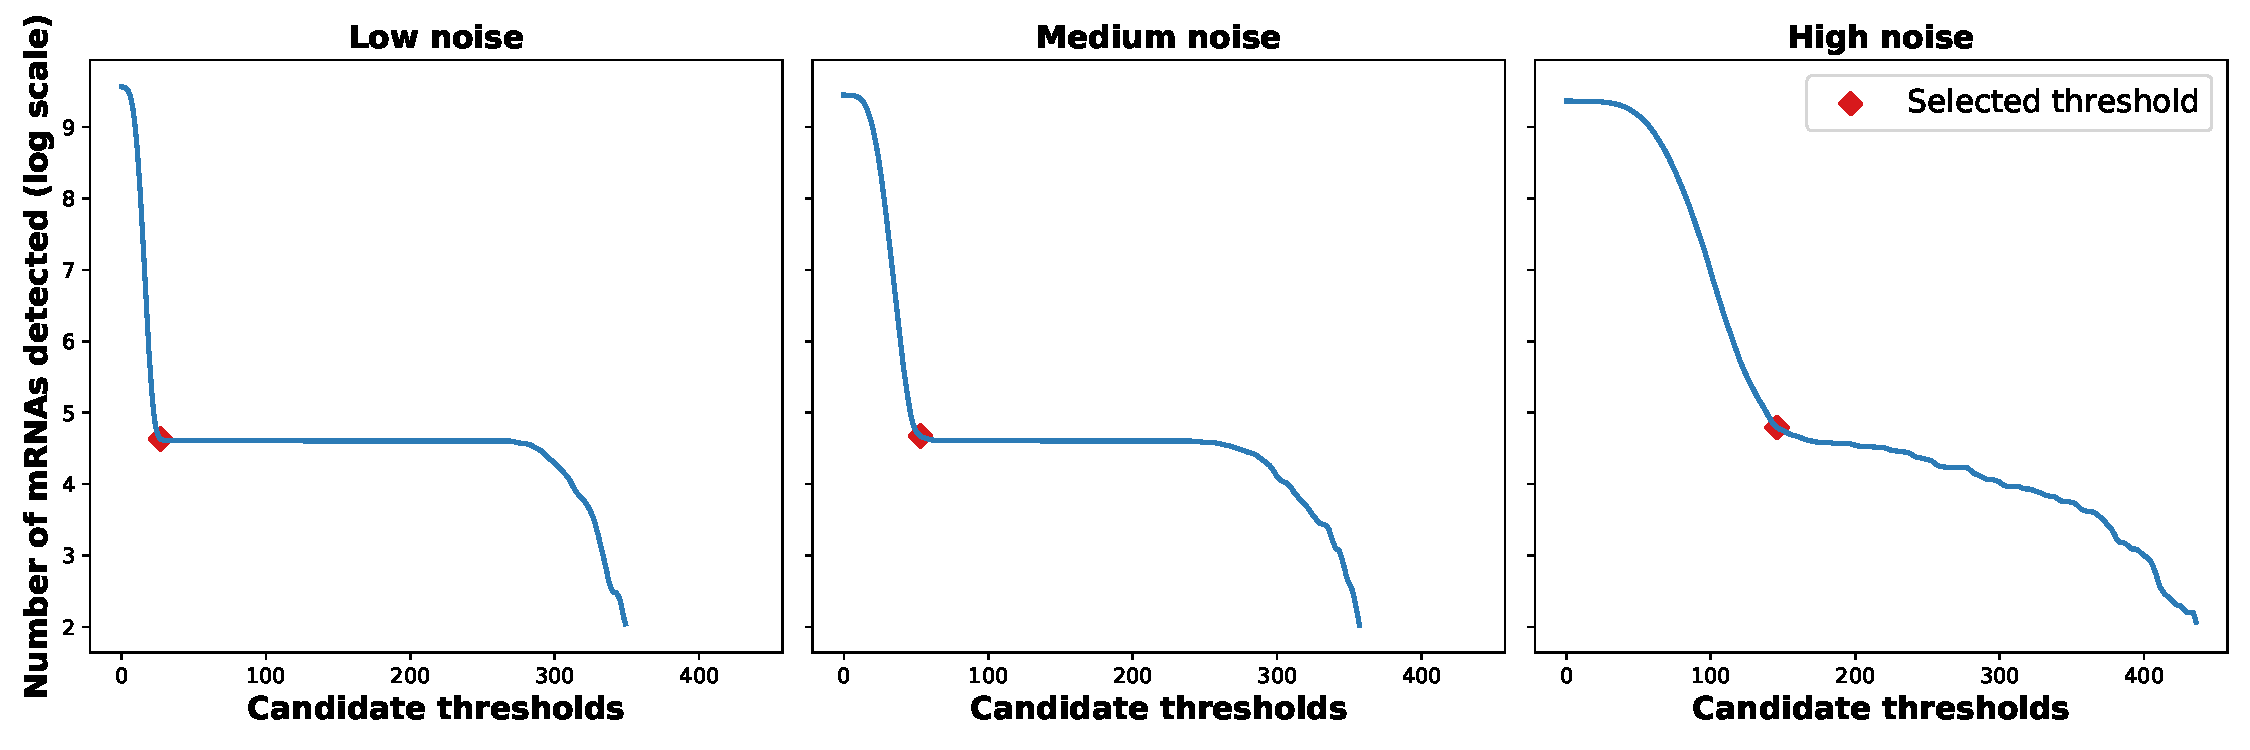
\includegraphics[width=1\textwidth]{figures/appendix/spots_elbow}
    \caption[Elbow curves with different noise levels]{Elbow curves with different noise levels}
    \label{fig:general_spots_elbow}
\end{figure}

\begin{figure}[h]
    \centering
    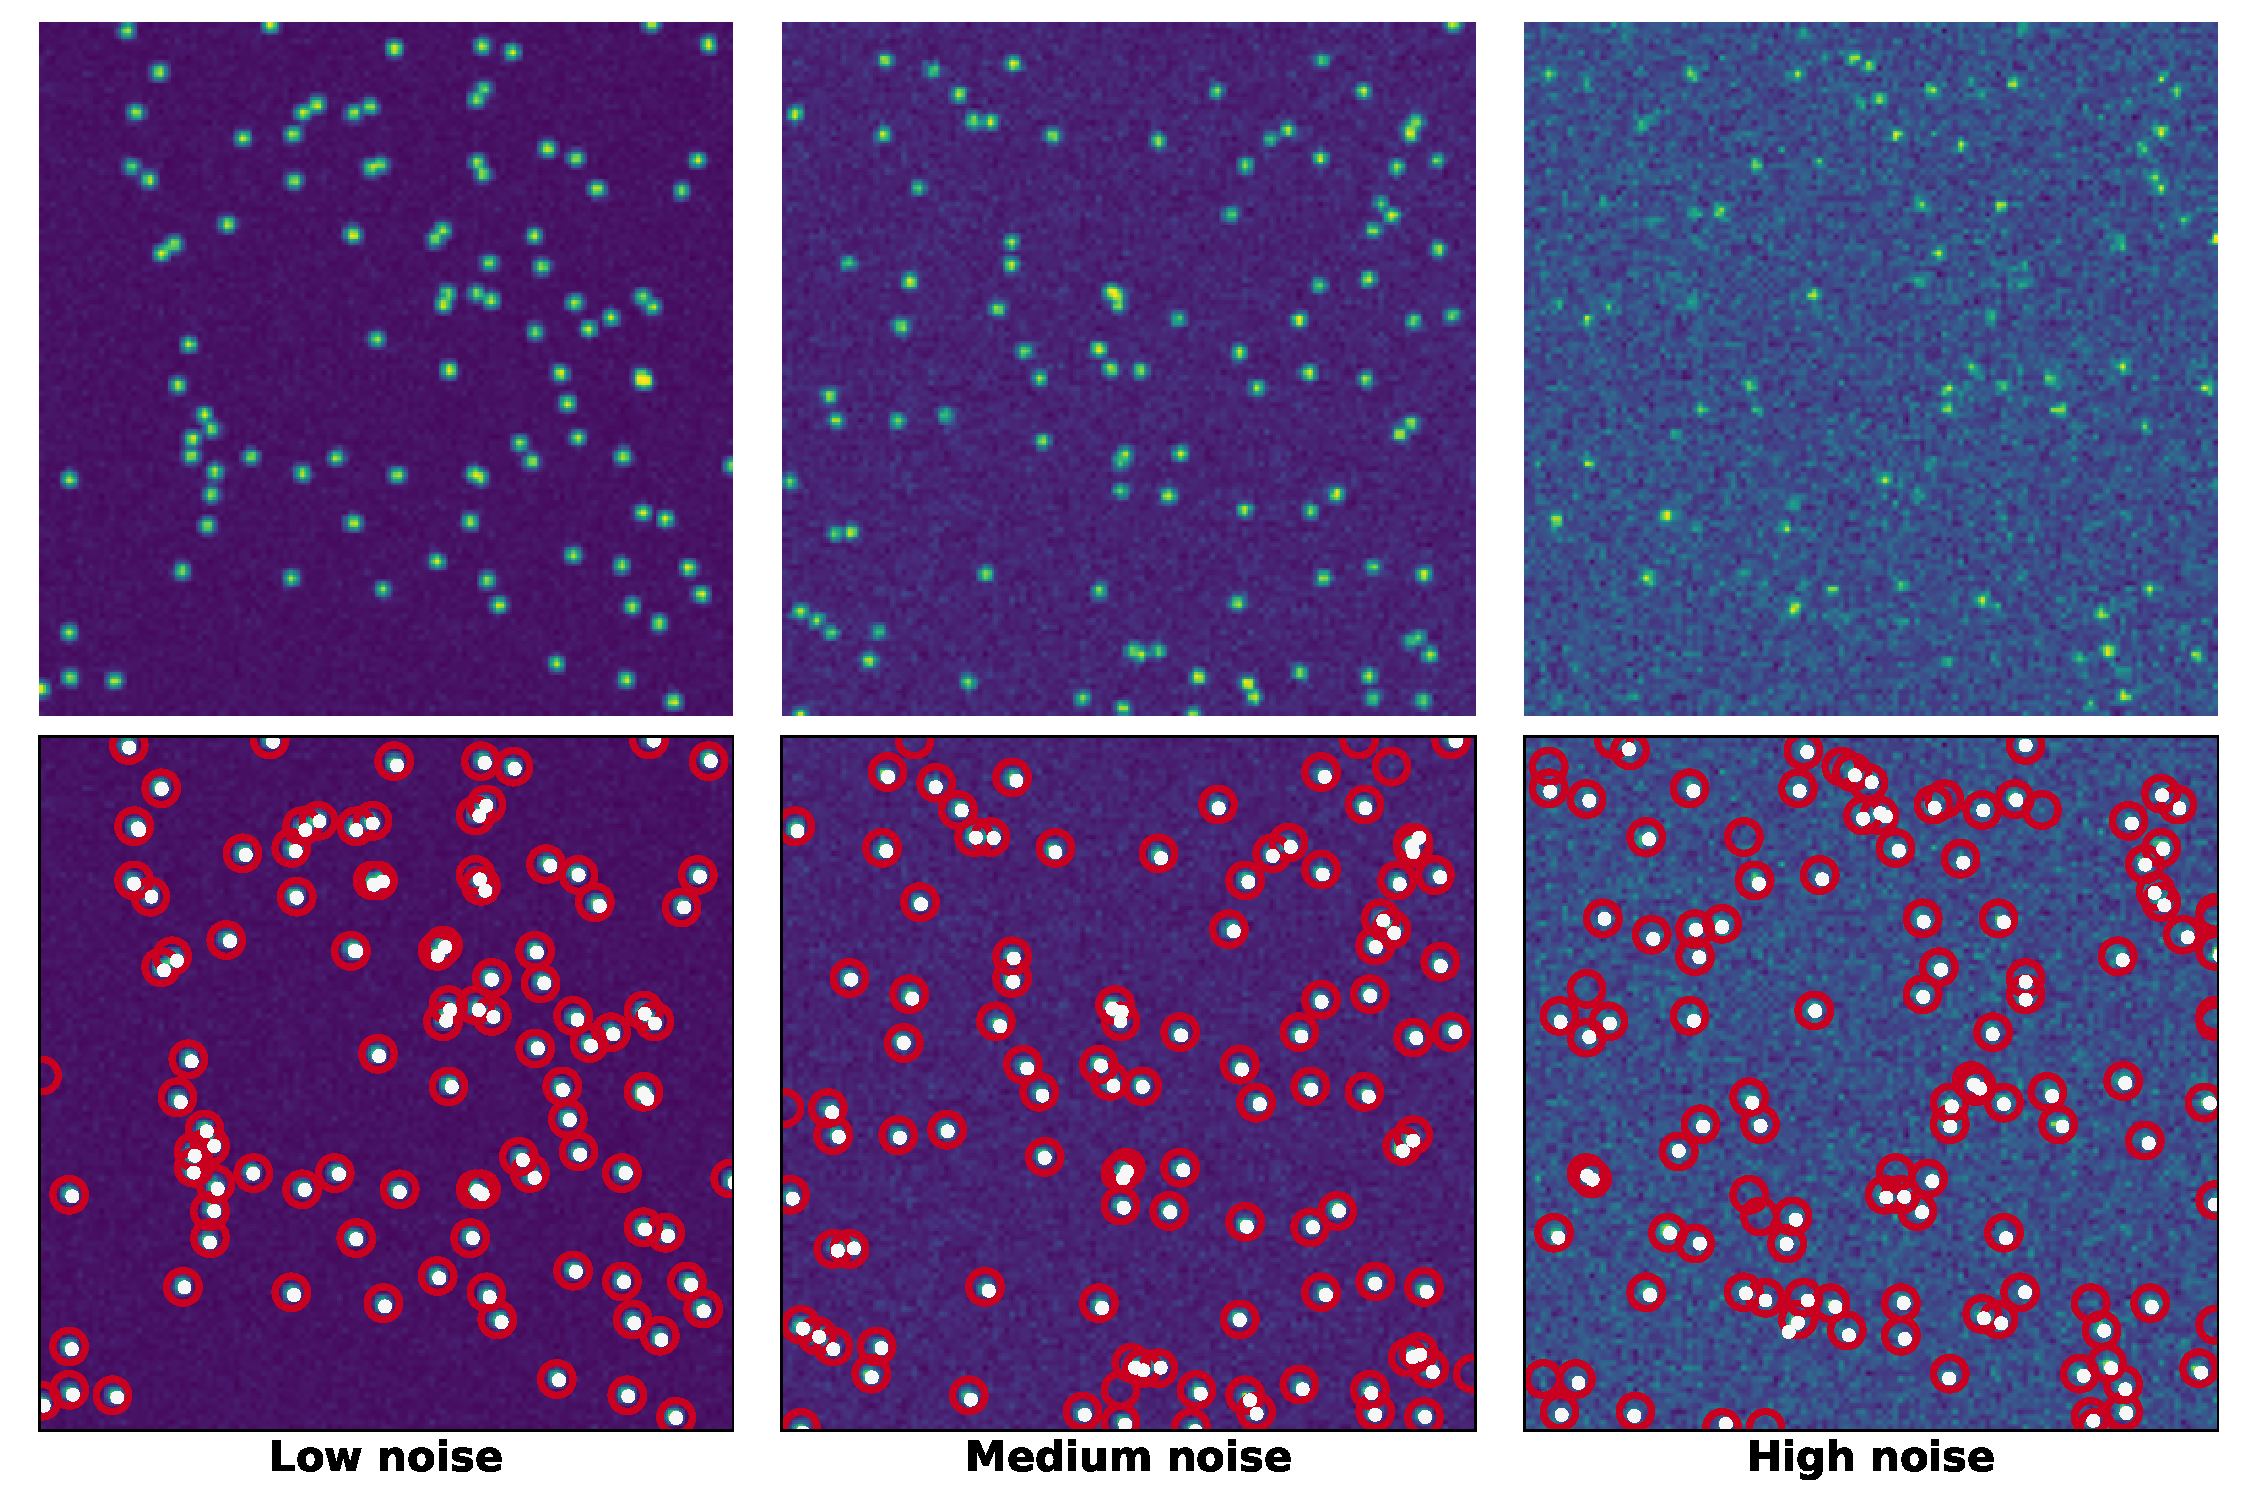
\includegraphics[width=1\textwidth]{figures/appendix/spots_example}
    \caption[Detection of 100 spots with different noise levels]{Detection of 100 spots with different noise levels}
    \label{fig:general_spots_detection}
\end{figure}
